% ::setlocal makeprg=cd\ presentazione\ &&\ pdflatex\ -interaction=batchmode\ main.tex\ &&\ xdg-open\ main.pdf\ &

\section{Capitolo 2}

\begin{frame}{Simulazione}

    Equazioni del moto per una particella massiva (unità adimensionali)

	\begin{align*}[left = {\empheqlbrace}]
        &\dv{\hat r}{\hat \tau} = \pm \sqrt{2 \mathcal E - 2 V_{\rm eff}} \\
        &\dv{\phi}{\hat \tau} = \frac{\hat \ell}{\hat r^2} \\
        &\dv{t}{\hat \tau} = \sqrt{2 \mathcal E + 1}
        \left(\frac{\hat r}{\hat r - 1}\right) 
	\end{align*}

    Si possono risolvere con \texttt{RK4}

\end{frame}


\begin{frame}{Caduta Radiale}

    $\hat \ell = 0$, $\mathcal E = 0$, $r_0 = 5$, $h = 10^{-4}$ \\
    Prompt: \texttt{./main.x 0 0 -r 5 -h 1e-4}

    \begin{figure}[h]
        \begin{minipage}{0.48\textwidth}
            \centering
            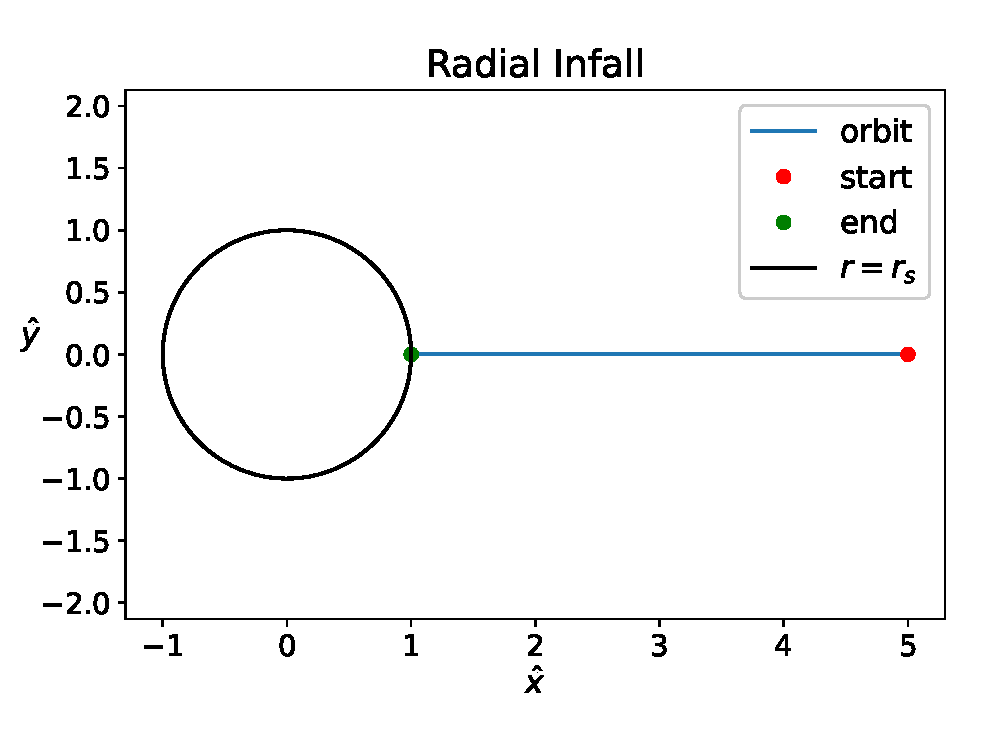
\includegraphics[width=\textwidth]{Figures/ch2/radial_infall.eps}
        \end{minipage}
        \hspace{0.015 \textwidth}
        \begin{minipage}{0.48\textwidth}
            \centering
            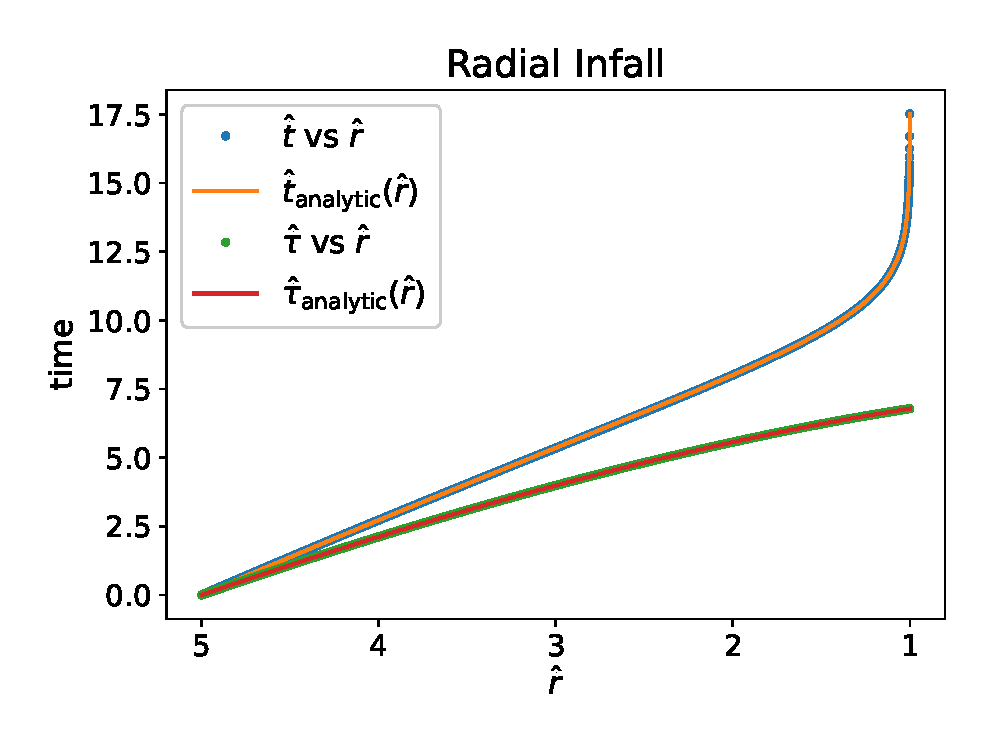
\includegraphics[width=\textwidth]{Figures/ch2/t_vs_tau.eps}
        \end{minipage}
    \end{figure}

\end{frame}


\begin{frame}{Caduta Radiale: Residui}

    $\hat \ell = 0$, $\mathcal E = 0$, $r_0 = 5$, $h = 10^{-4}$ \\
    Prompt: \texttt{./main.x 0 0 -r 5 -h 1e-4}

    \begin{figure}[h]
        \begin{minipage}{0.48\textwidth}
            \centering
            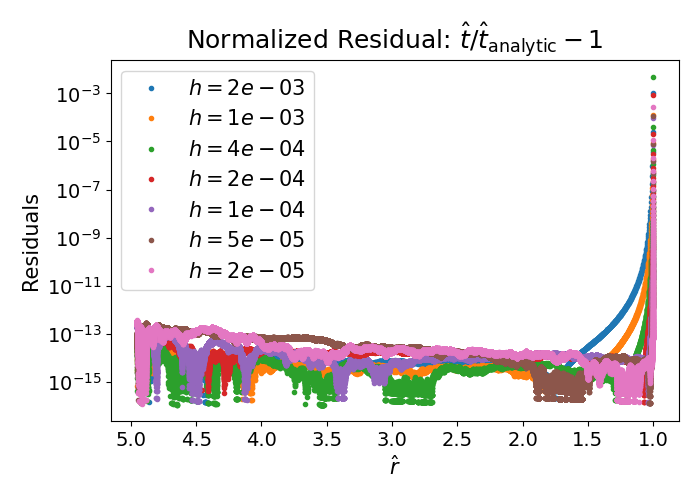
\includegraphics[width=\textwidth]{Figures/ch2/t_res_multi.png}
        \end{minipage}
        \hspace{0.015 \textwidth}
        \begin{minipage}{0.48\textwidth}
            \centering
            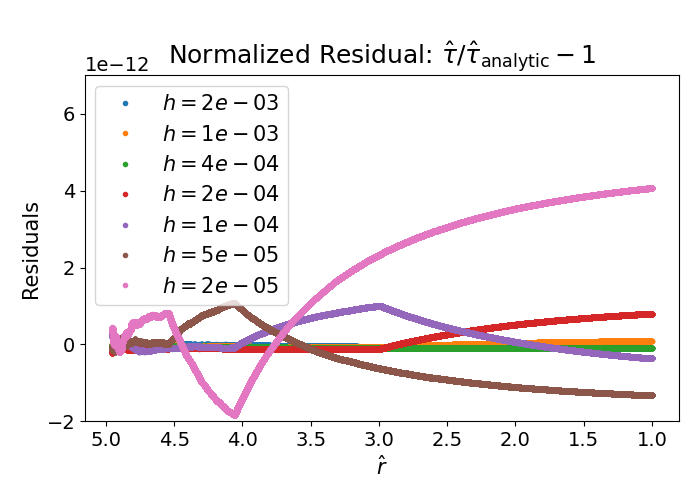
\includegraphics[width=\textwidth]{Figures/ch2/tau_res_multi.png}
        \end{minipage}
    \end{figure}

\end{frame}

\begin{frame}{Il Cambio di Segno}

    \begin{equation*}
        \dv{\hat r}{\hat \tau} = \pm \sqrt{2 \mathcal E - 2 V_{\rm eff}}
    \end{equation*}

    \texttt{
    double TESI\_fun\_r(double r, double E, double l, int *sign, int *Nturns)\{ \\
        ~~~~double foo = 2 * (E - TESI\_Veff(r, l)); \\
        ~~~~if (foo < 0)\{ \\
        ~~~~    ~~~~*sign *= -1; \\
        ~~~~    ~~~~*Nturns += 1; \\
        ~~~~\} \\
        ~~~~return *sign * pow(fabs(foo), 1. / 2.); \\
    \}
    }

\end{frame}


\begin{frame}{Casi Possibili, Scelta di $r_0$ e Segno}

    \begin{figure}
        \centering
        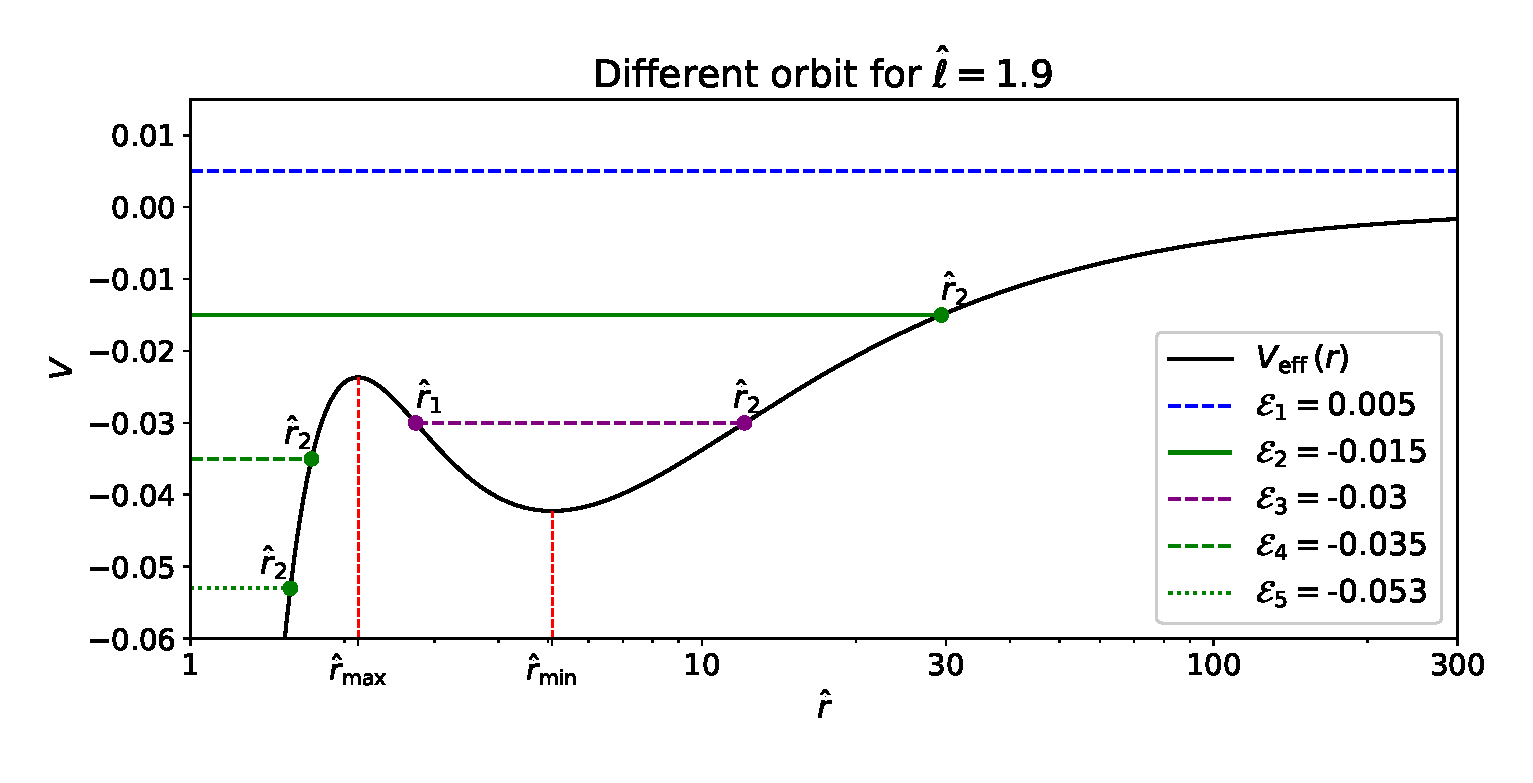
\includegraphics[width=0.9\textwidth]{Figures/ch2/scenario1.eps}
    \end{figure}

\end{frame}


\begin{frame}{Casi Possibili, Scelta di $r_0$ e Segno}

    \begin{figure}
        \centering
        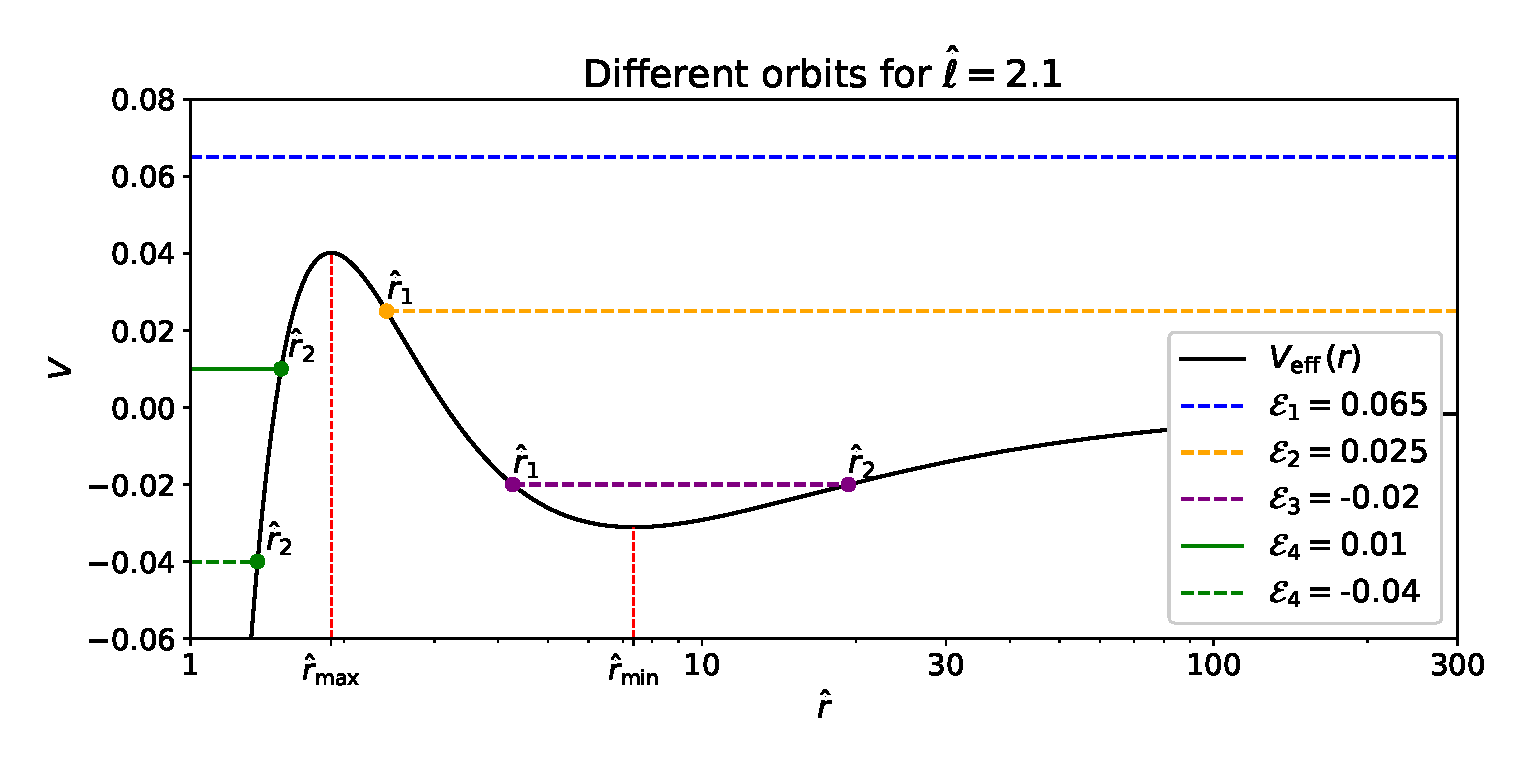
\includegraphics[width=0.9\textwidth]{Figures/ch2/scenario2.eps}
    \end{figure}

\end{frame}


\begin{frame}{Caduta 1}
    \centering
    \movie[externalviewer]{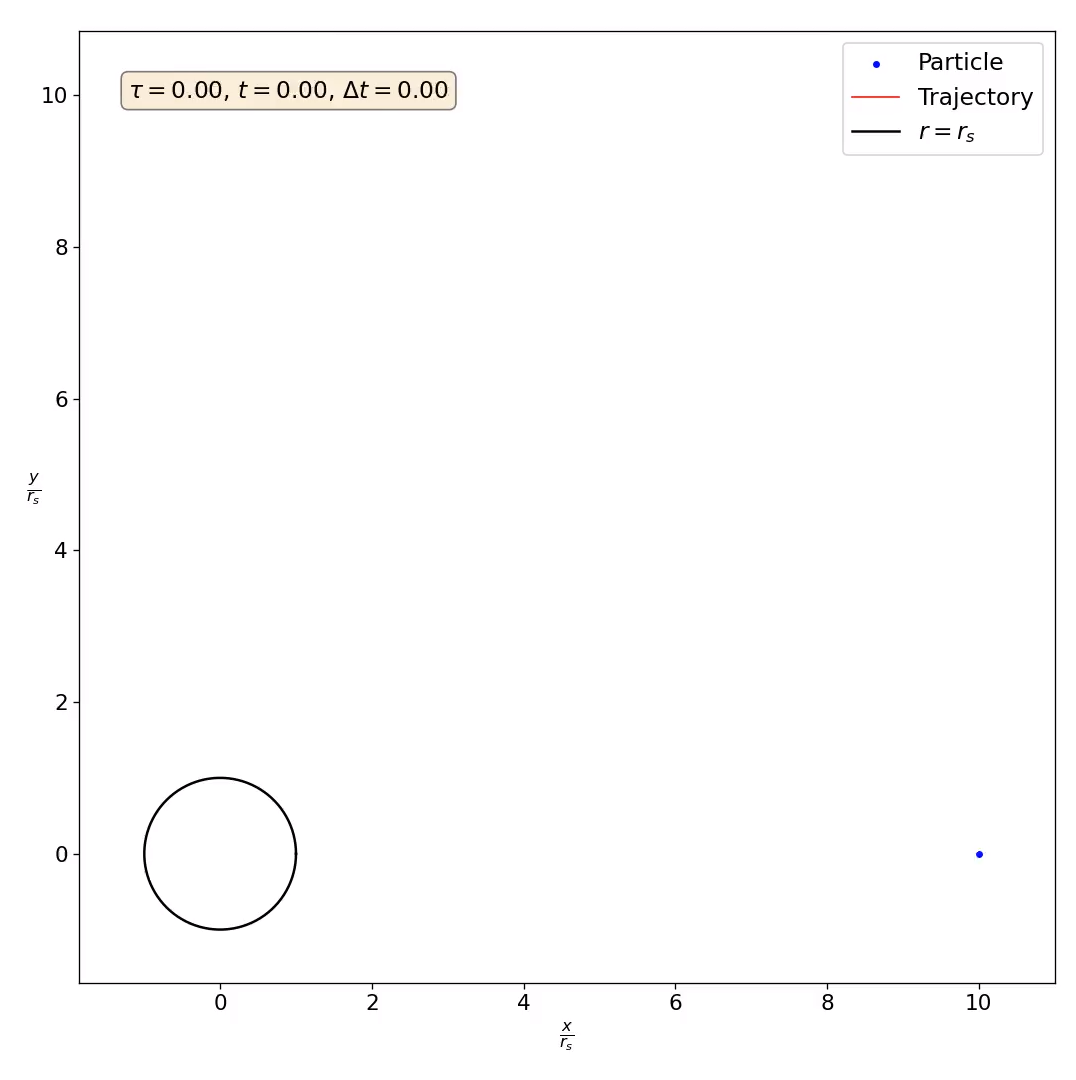
\includegraphics[width=\textheight, keepaspectratio]
    {Videos/infall.png}}{Videos/infall.mov}
\end{frame}


\begin{frame}{Caduta 2}
    \centering
    \movie[externalviewer]{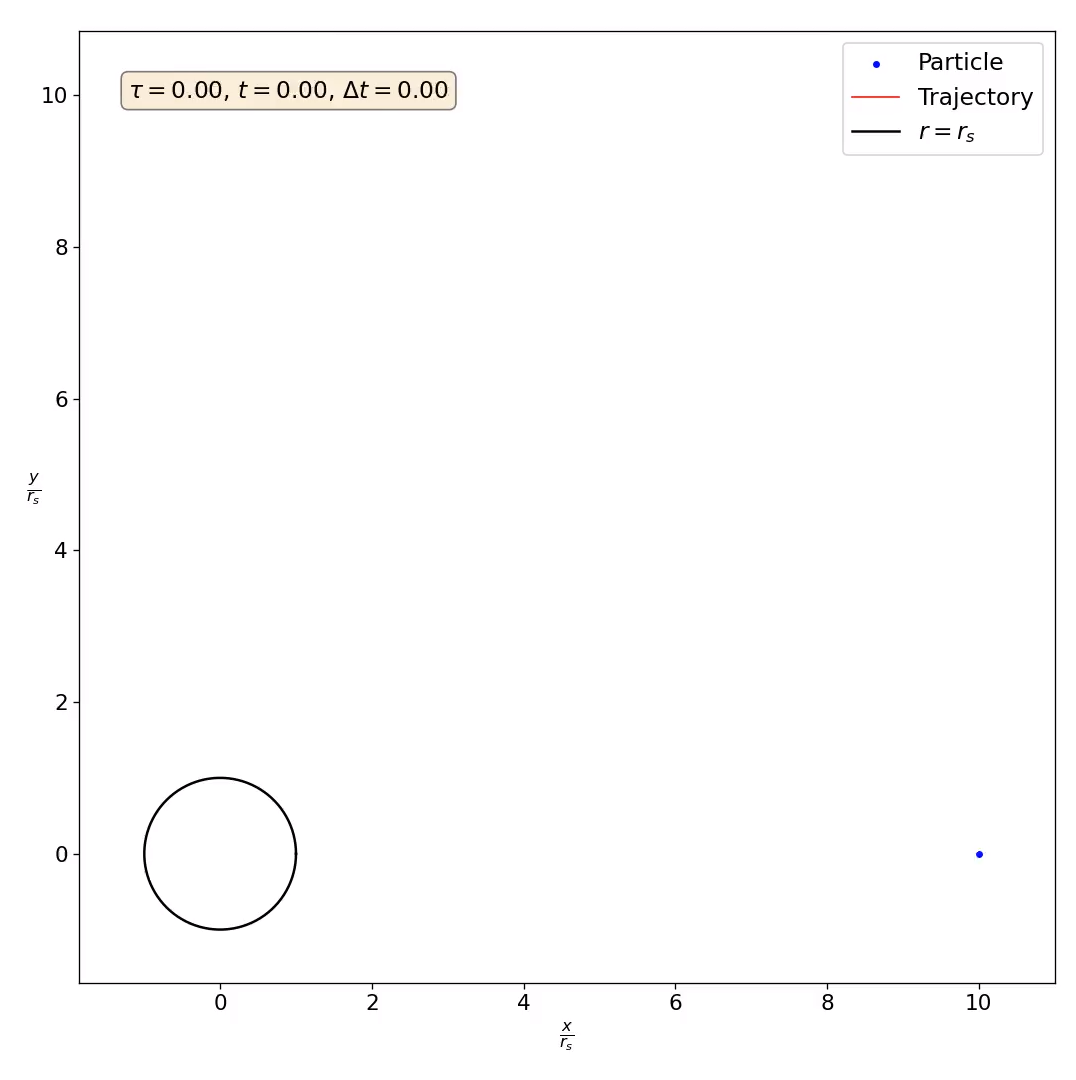
\includegraphics[width=\textheight, keepaspectratio]
    {Videos/infall.png}}{Videos/infall.mp4}
\end{frame}


\begin{frame}{Video on the computer}
    \centering
    \movie[externalviewer]{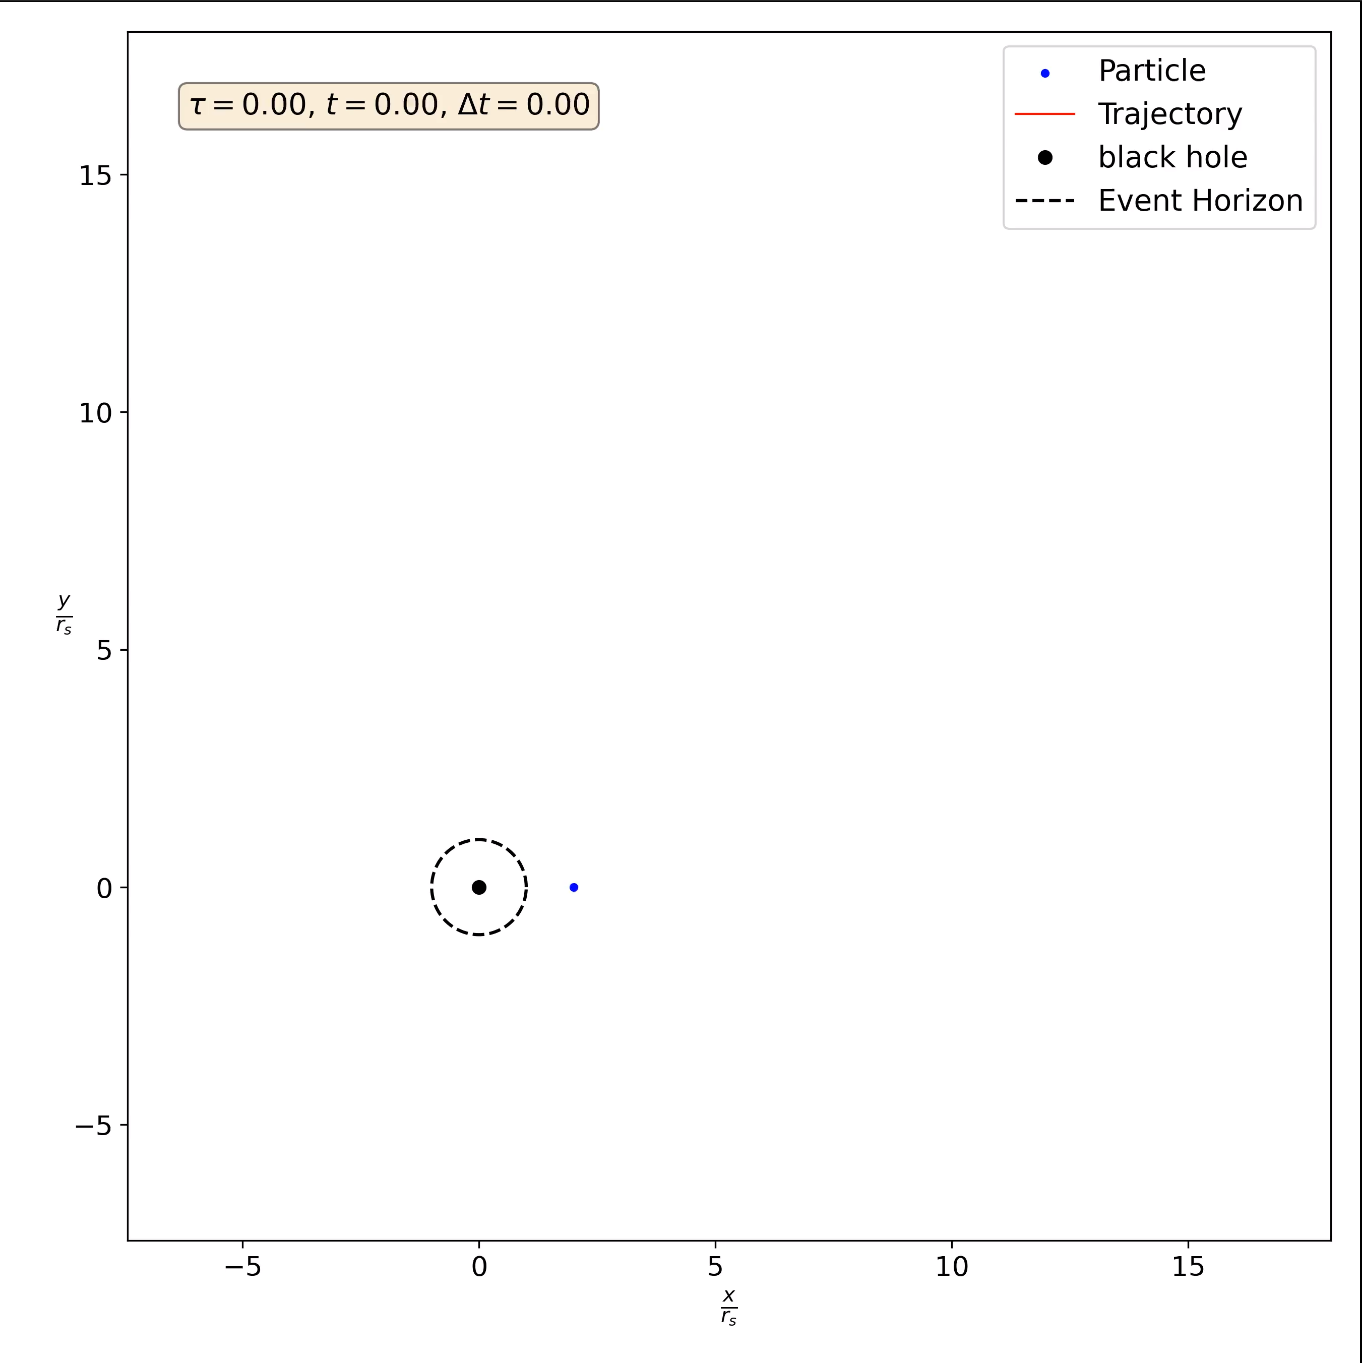
\includegraphics[width=\textheight, keepaspectratio]
    {Videos/volevi.png}}{Videos/volevi.mov}
\end{frame}


\begin{frame}{Video on the computer}
    \centering
    \movie[externalviewer]{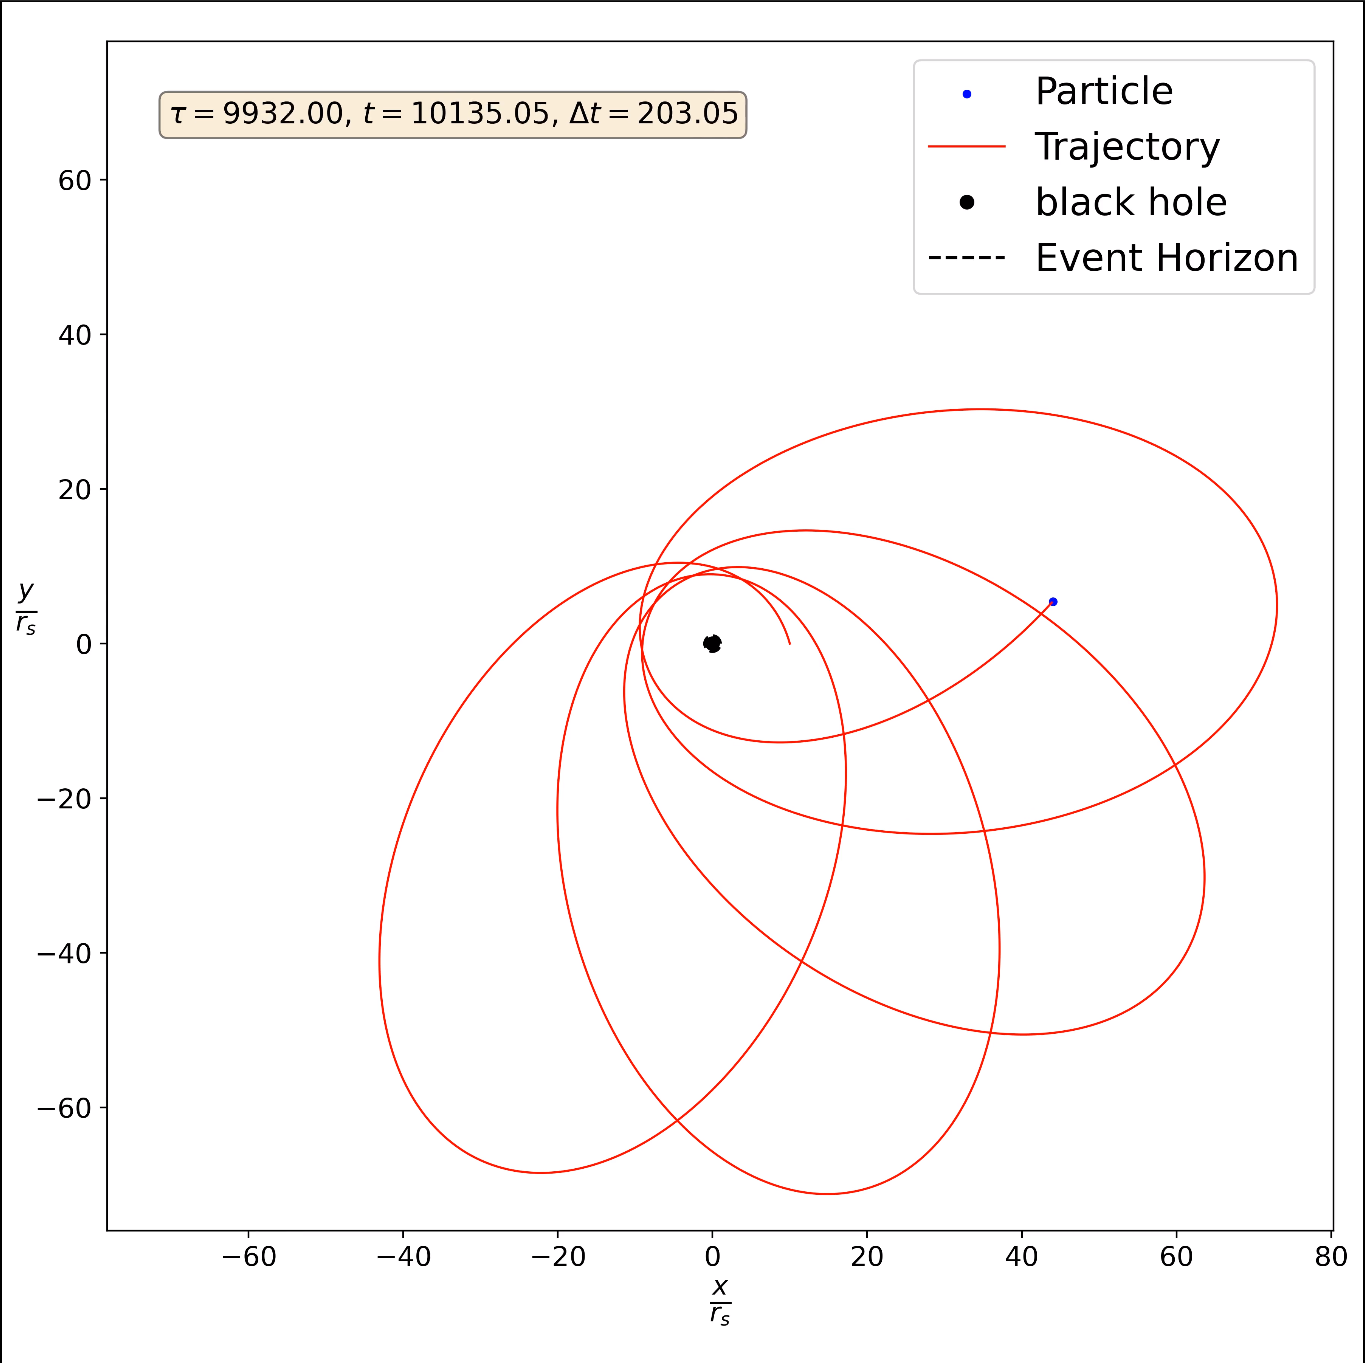
\includegraphics[width=\textheight, keepaspectratio]
    {Videos/precession.png}}{Videos/precession.mp4}
\end{frame}


\begin{frame}{Video on the computer}
    \centering
    \movie[externalviewer]{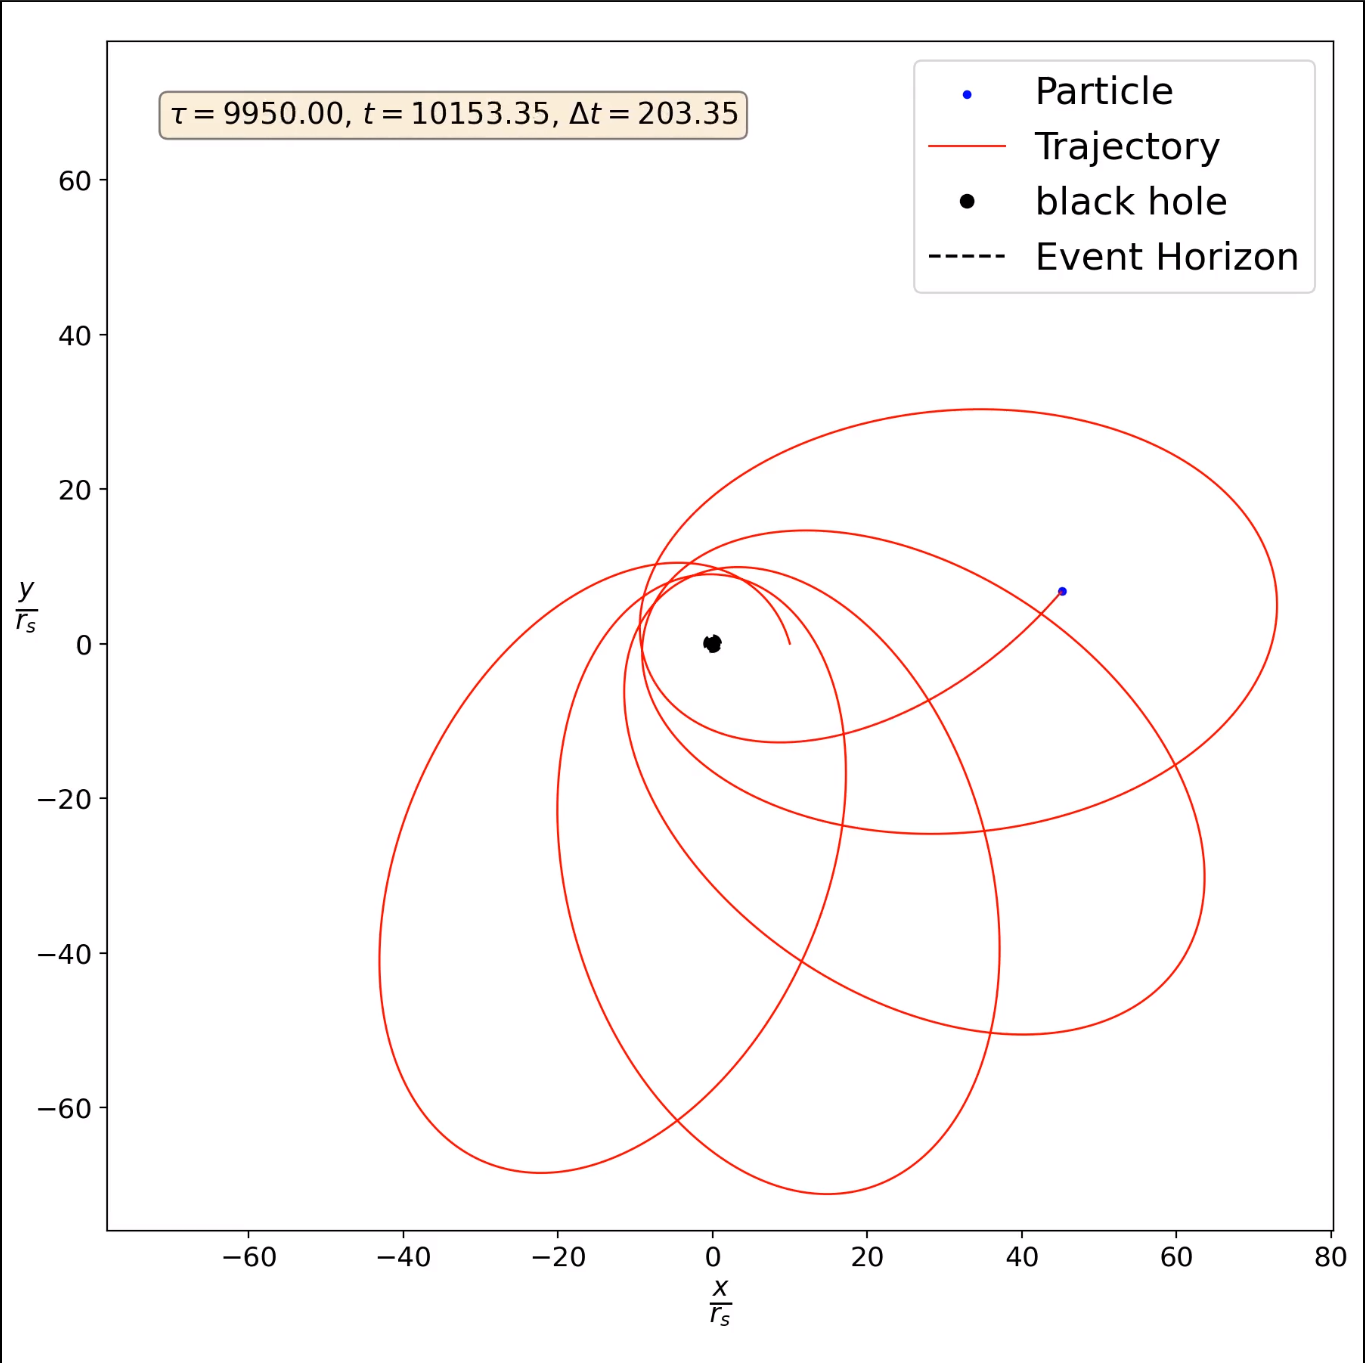
\includegraphics[width=\textheight, keepaspectratio]
    {Videos/precession2.png}}{Videos/precession2.mp4}
\end{frame}


\begin{frame}{Video on the computer}
    \centering
    \movie[externalviewer]{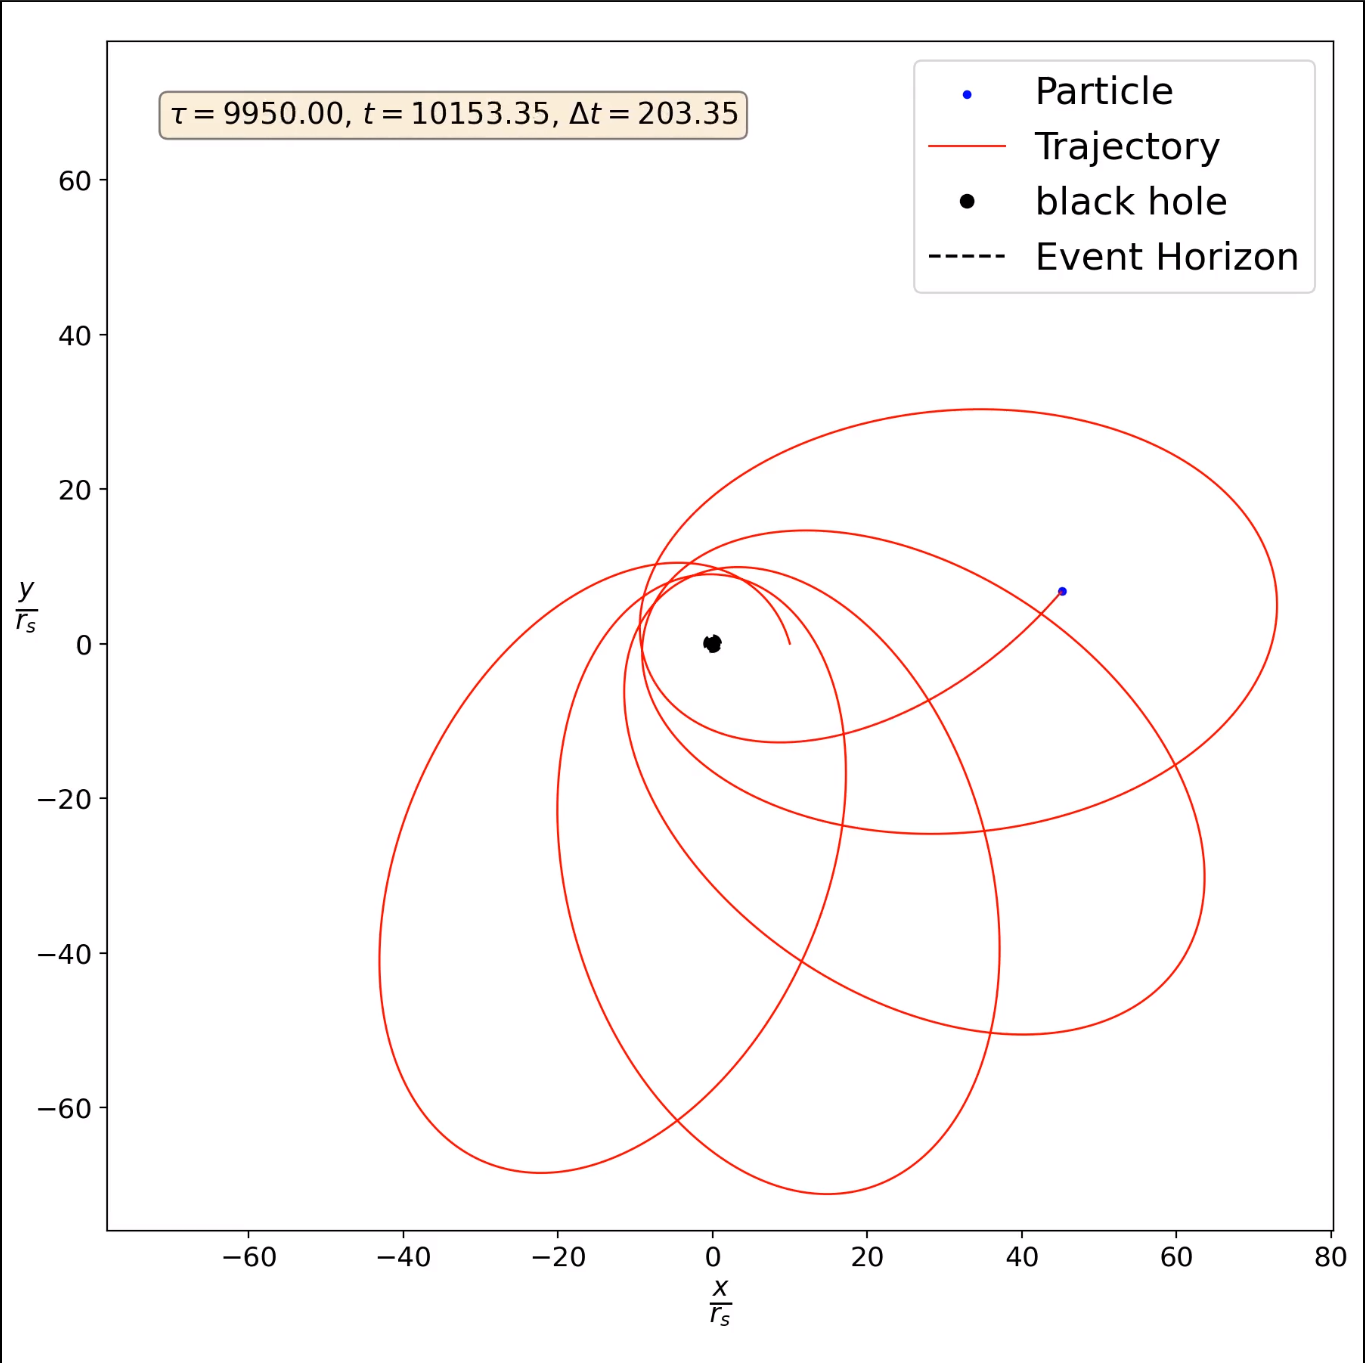
\includegraphics[width=\textheight, keepaspectratio]
    {Videos/precession2.png}}{Videos/precession2.MOV}
\end{frame}


\begin{frame}{Video on the computer}
    \centering
    \movie[externalviewer]{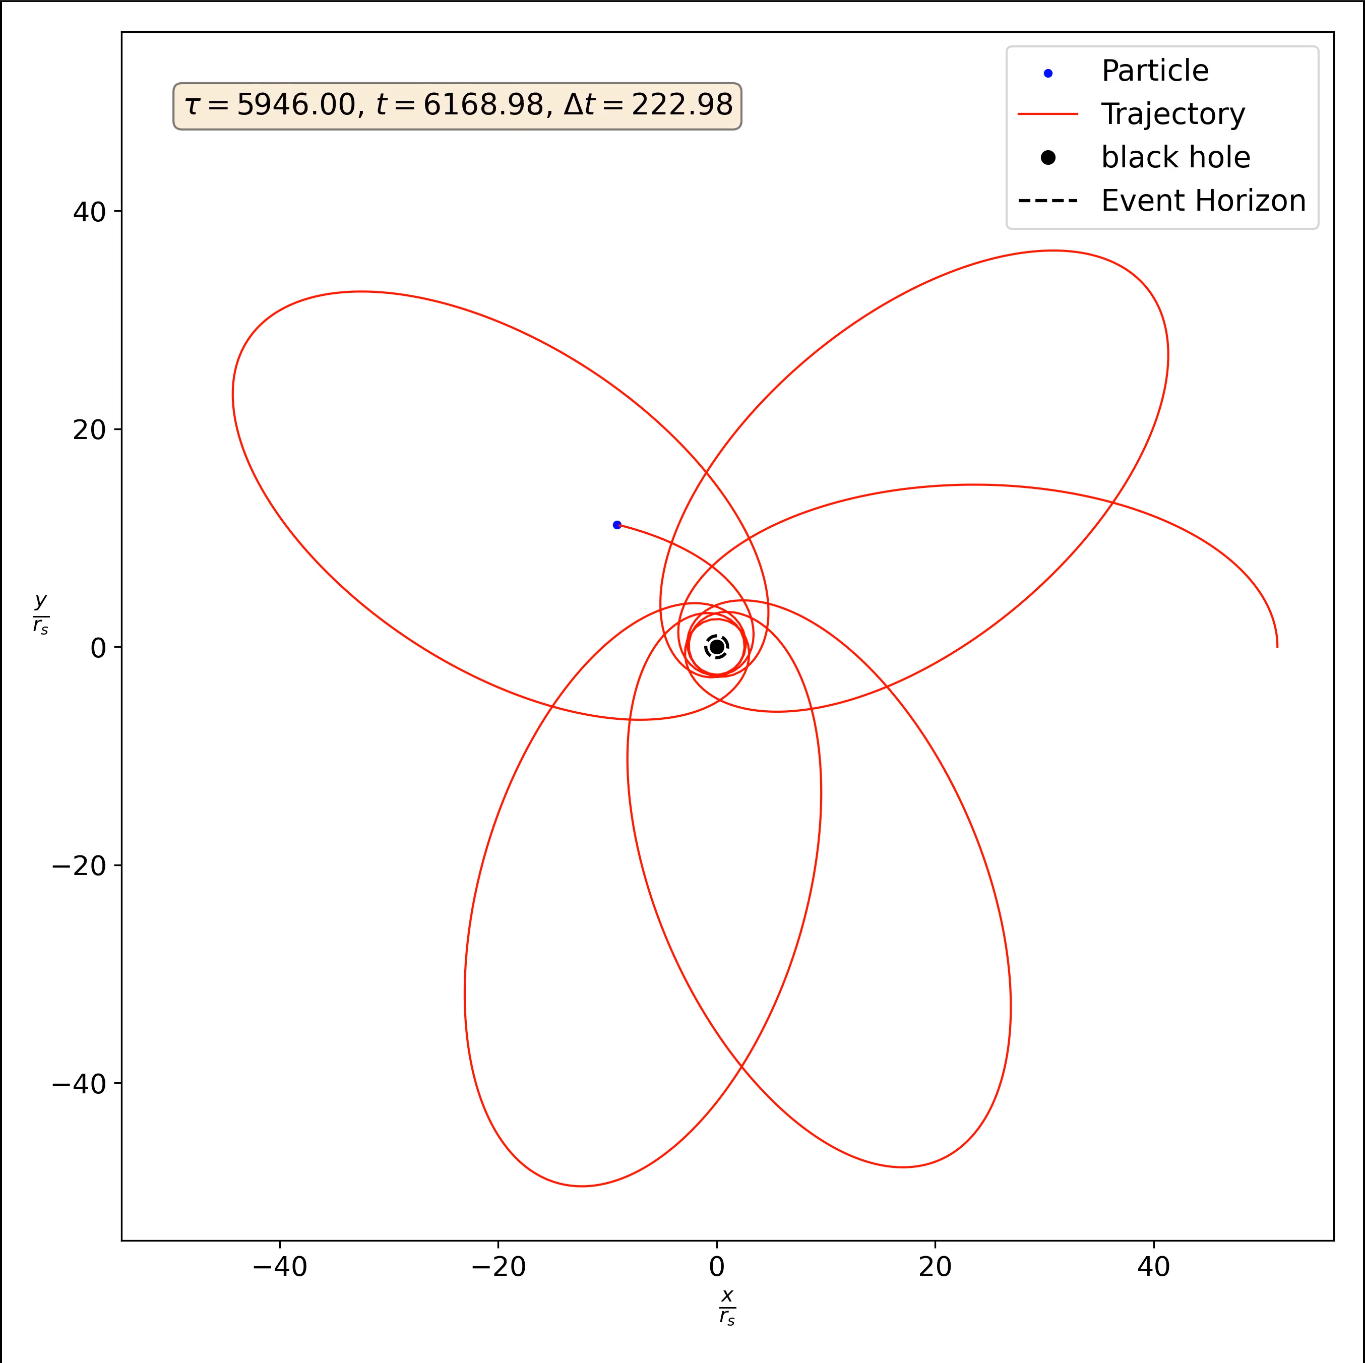
\includegraphics[width=\textheight, keepaspectratio]
    {Videos/precession_ani.png}}{Videos/precession_ani.mov}
\end{frame}
